\documentclass{VUMIFPSkursinis}
\usepackage{algorithmicx}
\usepackage{algorithm}
\usepackage{algpseudocode}
\usepackage{amsfonts}
\usepackage{amsmath}
\usepackage{array}
\usepackage{bm}
\usepackage{caption}
\usepackage{color}
\usepackage{float}
\usepackage{graphicx}
\usepackage{listings}
\usepackage{longtable}
\usepackage{subfig}
\usepackage{wrapfig}
\usepackage{enumitem}
\usepackage{pdfpages}

\usepackage[tableposition=top]{caption}
%PAKEISTA, tarpai tarp sąrašo elementų
\setitemize{noitemsep,topsep=0pt,parsep=0pt,partopsep=0pt}
\setenumerate{noitemsep,topsep=0pt,parsep=0pt,partopsep=0pt}

\newcolumntype{L}[1]{>{\raggedright\let\newline\\\arraybackslash\hspace{0pt}}m{#1}}
\newcolumntype{C}[1]{>{\centering\let\newline\\\arraybackslash\hspace{0pt}}m{#1}}
\newcolumntype{R}[1]{>{\raggedleft\let\newline\\\arraybackslash\hspace{0pt}}m{#1}}

% Titulinio aprašas
\university{Vilniaus universitetas}
\faculty{Matematikos ir informatikos fakultetas}
\department{Programų sistemų katedra}
\papertype{Praktikos ataskaita}
\title{Profesinės praktikos ataskaita}
\titleineng{Professional Internship Report}
\status{4 kurso 3 grupės studentas}
\author{Gediminas Krasauskas}
\supervisor{prof. dr. Romas Baronas}
\date{Vilnius – \the\year}

% Nustatymai
% \setmainfont{Palemonas-2.1}   % Pakeisti teksto šriftą į Palemonas (turi būti įdiegtas sistemoje)
\bibliography{bibliografija}

%--------------------------------------------------------
%----------------------- PRADŽIA ------------------------
%--------------------------------------------------------

\begin{document}
\maketitle
\tableofcontents

%--------------------------------------------------------
%------------------------ ĮVADAS ------------------------
%--------------------------------------------------------

\sectionnonum{Įvadas}
Praktika buvo atlikta UAB BPN LT media agentūros įmonės filiale Vilniuje. Vienintelę darbo patirtį prieš tai turėjau UAB Palink IKI prekybos tinkle kasininko-pardavėjo pozicijoje, tačiau to nebūtų galima pavadinti su profesija susijusia darbo patirtimi. Per visus studijų metus nesu dirbęs jokioje su IT susijusioje įmonėje, nes darbo paieškos baigdavosi labai nesėkmingai: darbo vietos nepavyko rasti nepaisant to, kad paieškos procesu užsiimu nuo pat 2 studijų semestro.

Noriu pasidžiaugti, kad privalomoji profesinė praktika yra Programų sistemų studijų programos dalis. Jaučiu, kad tik tokiu būdu galėjau rasti praktikos poziciją darbo rinkoje. Visą paieškos procesą palengvino praktikos internetinė sistema, kurioje buvo suteiktos sąlygos patogiai atsirinkti ir užsiregistruoti į sąraše esančias darbo pozicijas pokalbiui su darbdaviu.

Būtent jau minėtoje sistemoje radau savo praktikos atlikimo vietą. BPN LT nebuvo ta įmonė, kurioje maniau, kad atliksiu praktiką. Pagrindiniai kriterijai, renkantis praktikos vietą buvo:

\begin{enumerate}
    \item Alga. Kadangi turiu finansinių sunkumų, ieškojau pozicijos, kuri praktikantui siūlytų bent minimalų atlyginimą arba skiriamą premiją po praktikos.
    \item Galimybės kilti karjeros laiptais. Prioritetą kėliau didelėms korporacijoms, kurios turėtų aiškią hierarchiją ir tikimybę kilti hierarchijos laiptais, priklausomai nuo rodomų rezultatų.
    \item Įdomi veikla. Kadangi esu žmogus, nemėgstantis programavimo, ieškojau IT projektų vadovo, jo asistento, analitiko arba architekto pozicijų.
    \item Darbo sąlygos. Norėjau rasti praktiką, kurią būtų paprasta pasiekti viešuoju transportu, o pačioje įmonėje būtų jauku dirbti, sudarytos sąlygos poilsiui, bei įvairūs kiti privalumai.
\end{enumerate}
\bigskip

Praktikos paieškos laikotarpiu sudalyvavau 2 darbo pokalbiuose, tačiau nė viena įmonė neatitiko mano išankstinių reikalavimų. BPN LT pasirinkau dėl to, kad įmonę buvo paprasčiausia pasiekti viešuoju transportu (30-40 min. kelionės laiko).

Praktikos niuansų derinimo su darbdaviu eigoje trišaliu sutarimu buvo priimta praktikos tema ir jos uždaviniai. Tačiau po maždaug 5 savaičių nuspręsta juos pakeisti, nes vykdoma veikla įmonėje neatitiko pradinės temos ir uždavinių. Praktikos tema: „Skaitmeninės reklamos planavimo optimizacija“.

Praktikos atlikimo laikotarpiui buvo iškelti atlikti tokie uždaviniai:
\begin{itemize}
    \item Skaitmeninės reklamos planavimo proceso analizė.
    \item Skaitmeninės reklamos planavimo proceso analizės rezultatų įgyvendinimas.
\end{itemize}
\bigskip

Taip pat su darbdaviu aptartas ir nustatytas praktinės veiklos planas:
\begin{enumerate}
    \item Susipažinti su įmone, jos veiklos sritimi, struktūra ir naudojamomis technologijomis.
    \item Susipažinti su Google Apps Script technologija, jos dokumentacija bei platforma.
    \item Surinkti projektui keliamus reikalavimus iš įmonės projektų vadovų.
    \item Parengti pradinį projekto prototipą.
    \item Vystyti projektą iki galutinės veikiančios versijos pridedant naują funkcionalumą.
    \item Perduoti galutinį projektą kolegoms testuoti.
    \item Parengti projekto dokumentaciją.
    \item Įdiegti projektą visiems BPN darbuotojams.
\end{enumerate}
\bigskip

Pirmą praktikos dieną buvau supažindintas su įmonės aplinka: kolegomis, patalpomis, įmonės organizacine struktūra ir bendrąja tvarka. Po to buvo pristatyta mano darbo vieta ir reikiami įrankiai. Gavau prisijungimo duomenis prie asmeninio įmonės elektroninio pašto, kurį naudojau kaip pagrindinį komunikavimo su kolegomis įrankį. Toliau buvo suderintos su mano paskyra susijusios prieigos teisės.

Kitą dieną turėjau pokalbį su įmonės projektų vadovais, kurių darbą turėjau optimizuoti, bei pagrindiniu IT specialistu. Buvo aptarti jų lūkesčiai, projekto detalės, mano gebėjimai ir praktinės veiklos planas. 

Praktikos metu man teko išmokti dirbti su Google technologijomis: Google Apps Script, Google Sheets. Taip pat prireikė JavaScript, HTML bei UML žinių, kurias įgijau universitete.

Programuoti su Google Apps Script mokiausi rastuose internetinėse pamokose ir oficialioje technologijos dokumentacijoje. Kilus sunkumams į pagalbą pasitelkdavau dokumentaciją ir forumus, tokius kaip Stack Overflow.

Pirmas 2 savaites mokiausi dirbti su naujomis technologijomis. Nuo 3 iki 7 savaitės vykdžiau projekto realizaciją, programavau. 8 savaitę perdaviau sistemą kolegoms testuoti ir pradėjau dokumentuoti projektą. 9 savaitę atlikau testavimo metu kolegų rastas klaidas ir trūkumus, papildžiau funkcionalumą. Paskutinę savaitę baigiau projekto dokumentaciją ir diegiau projektą. Reikalavimų rinkimas buvo nuoseklus procesas, kurį vykdžiau viso praktikos laikotarpio metu.

Visą projektą nuo pradžios iki pabaigos dariau individualiai ir be jokių išorinių varžymų. Laikau tai vienu iš pagrindinių praktikos privalumų, nes turėjau visišką kūrybinę laisvę, galėjau susiplanuoti darbo procesą ir struktūrizuoti kodą savo nuožiūra.


%--------------------------------------------------------
%----------------------- DĖSTYMAS -----------------------
%--------------------------------------------------------

\section {Įmonės apibūdinimas}

Įmonė BPN LT įsikūrė 2015 m. Lietuvoje. Įmonės gyvavimo pradžioje dirbo 4 žmonės, tačiau spartus augimas lėmė, kad šiuo metu BPN LT dirba 32 darbuotojai. Įmonė taip pat yra tarptautinio tinklo IPG dalis. 

BPN LT misija - padėti klientams pasiekti augimą naudojant progresyvų, duomenimis paremtą turinį ir tikslinės auditorijos pasiekiamo metodus. 

Įmonė turi išsikėlusi ambicingus tikslus: 
\begin{itemize}
    \item Tapti geriausiai klientus aptarnaujančia agentūra rinkoje.
    \item Tapti \#1 (pagal apyvartą) agentūra Baltijos šalyse.
    \item Būti lyderiu DIGITAL \& DATA kompetencijose.
\end{itemize}
\bigskip

Ambicingumas ir siekiami rezultatai padėjo įmonei pasiekti pripažintų rezultatų: 
\begin{itemize}
    \item BPN LT - 3 metus iš eilės sparčiausiai auganti agentūra.
    \item Įmonė aptarnauja apie 40 klientų.
\end{itemize}
\bigskip

Toliau apibūdinama pagrindinė įmonės veiklos sritis, teikiamos paslaugos, organizacinė struktūra bei praktikos vietoje sudarytos darbo sąlygos.

\subsection{Veiklos sritis ir teikiamos paslaugos}
Pagrindinė veikla - media planavimas ir pirkimai. Įmonė pagal klientų poreikius sukuria Media planus bei juos optimizuoja. Sudėtinės šių darbų veiklos - reklamos kampanijų priežiūra pasiūlant sprendimus ir korekcijas bei tinkamiausių reklamos kanalų klientui atranka.

Papildomos įmonės veiklos ir paslaugos:
\begin{itemize}
    \item ROI modelių kūrimas;
    \item komunikacijos strategijos;
    \item elektroninės komercijos komunikacija;
    \item turinio rinkodara;
    \item didžiųjų duomenų analitika;
    \item media inovacijos;
    \item eksporto reklamos paslaugos;
    \item profesionalios SEO paslaugos.
\end{itemize}


\subsection{Organizacinė struktūra}
įmonėje dirba 32 darbuotojai.
3 iš jų direktoriai: media direktorius, strategijų direktorius ir įmonės vystymo direktorius (pagrindinis direktorius).
Didžioji dalis darbuotojų yra atskirų projektų vadovai: kampanijų vadovai, socialiniai vadovai ir turinio vadovai. Įmonėje taip pat dirba analitikai, administratorė ir buhalterė. Įmonė samdo vieną IT specialistą neterminuotam darbui. Kai kurie darbuotojai turi daugiau negu vieną rolę. Pavyzdžiui, administratorė yra ir analitikė.

Atskaitomumo ryšiai įmonėje nėra aiškiai apibrėžti, nes dauguma darbuotojų yra vadovai, atsakingi už konkrečius projektus, klientus arba veiklas. Paprastai darbuotojai yra suskirstomi į mažas komandas. Komandų gyvavimo ciklas būna trumpas, o komandų struktūra vis skirtinga, ir projektui pasibaigus komandos išyra. Įmonės hierarchija pavaizduota 1 pav.

\subsection{Praktikos vietoje sudarytos darbo sąlygos}
Įmonė suteikė darbo vietą Vilniaus biure, A. Tumėno g. 4. Biuro lokacija buvo gera - ją viešuoju transportu  pasiekdavau per 20-25 minučių. Kadangi įmonė yra įsikūrusi cente, prie pat Lietuvos Respublikos seimo, kelių šimtų metrų spinduliu yra labai platus spektras maitinimo įstaigų. Tiesa, kadangi algos man įmonė nemokėjo, tekdavo atsinešti namie pasigamintą maistą.

Tam, kad būtų galima patekti į biurą, reikėjo specialios kortelės, kurią nuskaičius specialiu elektroniniu prietaisu ant durų, jos atsirakindavo. Visos praktikos metu negavau jokios kortelės, todėl kas kart, norint patekti į biurą, turėdavau paskambinti skambučiu ir laukti, kol kuris nors darbuotojas, dažniausiai administratorė, atrakins duris. Kortelės neišdavimą darbdavys argumentavo tuo, kad tos kortelės greitai pasimeta.

Įmonė darbuotojams parūpina visavertę darbo vietą: stalą, kėdę, darbinį nešiojamąjį kompiuterį, monitorių, klaviatūrą ir pelę. Tiesa, praktikai įsibėgėjus jautėsi darbo vietų trūkumas, nes kai kurie darbuotojai, tarp jų ir aš, buvo persodinami į kitas darbo vietas, o kai kurie ėjo dirbti į poilsio kambarį. Visame biure veikė interneto prieiga per Wi-Fi tinklą, tačiau būdavo dienų, kai internetas neveikdavo visą darbo dieną. Tokiais atvejais darbuotojai naudodavo savo mobilaus telefono interneto ryšio tikėjo duomenis. Kadangi aš negalėjau sau leisti šios prabangos, dirbdavau be interneto arba grįždavau namo ir dirbdavau iš ten.

Įmonės veikla buvo paskirstyta per 2 aukštus. Pirmame aukšte buvo laiptai į antrą aukštą. Abu aukštai turėjo po tualetą, o antrame aukšte buvo nedidelė virtuvė su kavos aparatu. Virtuvės reikmenimis buvo galima naudotis laisvai: bet kada pasidaryti kavos, pasišildyti vandenį ar maistą mikrobangų krosnelėje, pasinaudoti lėkštėmis, puodeliais bei šaldytuvu. Kartais buvo atvežama vaisių ir saldainių, kuriuos iš įmonės „Barbora“ užsakydavo darbovietė.

Darbuotojai, atvažiuojantys į darbą savo automobiliais galėjo jį pastatyti automobilių stovėjimo aikštelėje, pasiekiamą tiesiogiai iš antrame aukšte įsikūrusios virtuvės. Nors ir neturėjau automobilio, tai atrodė patogu.

Antrame aukšte taip pat buvo patalpa, skirta poilsiui bei veiklai su Play Station 4 žaidimų konsole, tačiau vėliau, dėl man nežinomų priežasčių, po kelių savaičių ji buvo pašalinta. Visi darbuotojai dirbo atviroje erdvėje su gera akustika, todėl buvo paprasta komunikuoti gyvai tarp darbuotojų, dirbančių tiek 1, tiek 2 aukšte. Tiesa, jautėsi tam tikra atskirtis, nes įmonės pagrindinio direktoriaus darbo vieta buvo atskira nuo visų darbuotojų ir joje buvo langas, pro kurį buvo galima stebėti visus darbuotojus.

Bendra atmosfera buvo ganėtinai jauki ir draugiška. Kolegos mane pasitiko neutraliai, tačiau nevengdavo bendrauti, pajuokauti. Tiesa, dėl geros akustikos ir dažnų šnekų tiek darbo, tiek neformaliais klausimais viskas girdėdavosi, o tai darydavo įtaką produktyvumui ir koncentracijai, kildavo sunkumų susikaupti. Be to, kartais grodavo muzika arba radijas per kolonėles lubose. Tačiau prie tokios atmosferos po kiek laiko pripratau ir visi išvardyti trukdžiai turėjo mažiau įtakos mano produktyvumui.

Apskritai biure tvyrojo jausmas, kad galima daryti labai daug. Vieni kolegos atsivesdavo savo augintinius šunis ir vaikus. Darbuotojai bet kuriuo metu išeidavo rūkyti, pietų laikas nebuvo stebimas, darbo kompiuteriuose buvo galima naršyti socialinius tinklus, klausytis muzikos.

Bendradarbiai organizuodavo vakarėlius, išvykas ir kitus renginius, kviesdavo į juos visą kolektyvą. Buvo švenčiami gimtadieniai, verslo pasiekimai ir kitos progos, kurių metu būdavo nuperkamos picos, tortai, gaivieji gėrimai, atsitraukiama nuo darbų ir bendrai švenčiama virtuvėje.

Darbo laikas būdavo tikrai lankstus, galima ateiti į biurą asmeniškai patogiu laiku. Ne kartą teko pasinaudoti galimybe dirbti iš namų nesant galimybėms atvykti į biurą.

\begin{figure}[H]
    \centering
    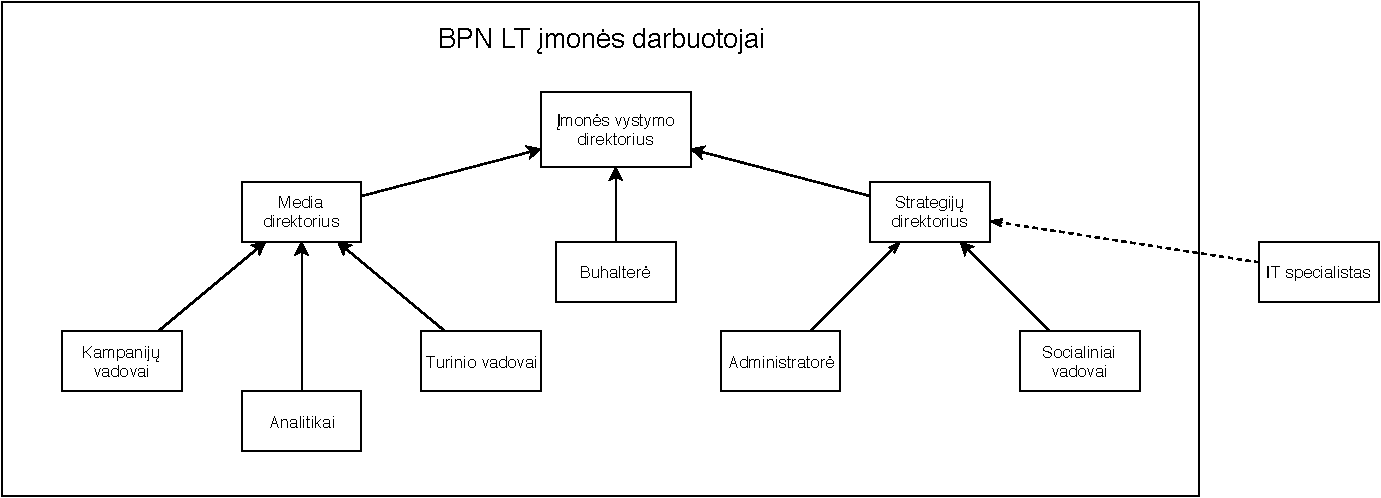
\includegraphics[scale=0.7]{img/organisational.pdf}
    \caption{įmonės organizacinė struktūra}
    \label{img:model}
\end{figure}

\section{Praktikos veiklos aprašymas}

\subsection{Informacijos šaltiniai}
Visą pagrindinę informaciją gaudavau iš oficialios Google Apps Script dokumentacijos. Ši dokumentacija yra patalpinta Google Apps Script interneto svetainėje. Ji buvo nepaprastai išsami, nes joje galėjau rasti visas funkcijas, jų aprašymus ir panaudojimo pavyzdžius.

Bendradarbių žinios. Be savo tiesioginio darbo vadovo dar bendravau su dalykinės srities ir IT atstovais, su kuriais galėjau konsultuotis atitinkamais klausimais. Dalykinės srities atstovas padėjo susigaudyti dalykinėje srityje: koks projektų vadovo tikslas, kokius šablonus jis pildo, kokias reikšmes ir kada pildo tuose šablonuose ir t.t. Tai man leido suprasti projekto poreikius ir jam keliamus reikalavimus. Šį konsultantą galėjau pasiekti bet kuriuo darbo dienos metu gyvai biure. Tai buvo labai patogu, nes didžioji dalis neaiškumų kildavo būtent iš dalykinės srities.

IT srities atstovas teikdavo konsultacijas IT klausimais: kokius algoritmus geriau parinkti, kokie sprendimai logiškesni, kur ieškoti informacijos. Jis taip pat suteikdavo pagalbą architektūriniais klausimais, t.y. kokią duomenų saugyklą parinkti, kaip įdiegti projektą ir pan. Tiesa, su šiuo žmogumi bendraudavau retai, nes biure jis pasirodydavo epizodiškai. Dėl to pagrindinis komunikavimo su juo būdas būdavo el. paštas. 

Nors šie darbuotojai ir teikdavo konsultacijas, galutinis verdiktas ir sprendimas buvo mano rankose. Išklausęs patarimus ir pasiūlymus visada priimdavau mano galva logiškiausius sprendimus.

Įvairūs internetiniai puslapiai padėjo rasti atsakymus į klausimus, kurių nerasdavau nei dokumentacijoje, nei pabendravęs su konsultantais. Teko pasinaudoti informacijos apsikeitimo tinklapiais, tokiais Stack Overflow ir Google Apps Script forumais. Taip pat programinio kodo pavyzdžiais kodo talpykloje GitHub. Vaizdo įrašais praktikos tematika YouTube, straipsniais Medium bei daugeliu individualių žmonių rašomų blogų.

\subsection{Praktikos tikslų įgyvendinimas}

Universitete įgytos bei praktikos pradžioje išmoktos žinios labai padėjo įgyvendinti projektą sėkmingai. Pirmoji užduotis buvo aptarti kokį projekto vadovo procesą automatizuosiu ir nuspręsti architektūrinį bei technologinį jo aspektus. Visa tai buvo aptarta privačiame pokalbyje su dalykinės ir IT srities konsultantais. Buvo nuspręsta, kad atliksiu skaitmeninės reklamos planavimo optimizaciją, naudojant Google Apps Script programavimo kalbą. Taip pat bendrai nutarėme, kad duomenų bazės įrašai bus patalpinti Google Spreadsheets skaičiuoklės atskirame faile. Galiausiai apsibrėžėme, kad visi kiti procesai bus atliekami pagal mano nuožiūrą: planavimas, reikalavimų analizė, programavimas, dokumentavimas ir diegimas. Testavimą atliks kolegos projektų vadovai, kurie atlieka skaitmeninės reklamos planavimą.

Toliau sekė mano individualus visos veiklos praktikos laikotarpiu planavimas. Planuoti buvo ypatingai įdomu, nes nuo planavimo kokybės tiesiogiai priklausė praktikos rezultatų sėkmė. Suplanavau, kad reikalavimus rinksiu visos praktikos metu, išskyrus paskutines 2 savaites. Pirmas 2 savaites mokysiuosi ir gilinsiuosi į Google Apps Script kalbą, toliau kitas 5 savaites programuosiu, 8-9 savaitę dokumentuosiu projektą bei duosiu jį testuoti kolegoms, taisysiu jų rastas klaidas, atsižvelgsiu į pastebėjimus, o 10 savaitę diegsiu projektą. Sukurtas planas konsultantus ir praktikos vadovą iš organizacijos pusės tenkino, o plano laikytis sekėsi itin sėkmingai - tik su kelių dienų paklaida. Plano lentelė pavaizduota žemiau.

\begin{table}[htb]
\centering
\caption{Praktikos bendrasis planas}
\begin{tabular}{|L{3.5cm}|L{12cm}|}
\hline

Laikotarpis (sav.) & 
Vykdoma veikla     
\\ \hline

1-8 & 
Projektui keliamų reikalavimų analizė.
\\ \hline

1-2 & 
Mokysis ir gilinimasis į Google Apps Script kalbą.  
\\ \hline

3-7 & 
Programavimas Google Apps Script kalba.
\\ \hline

8-9 & 
Projekto dokumentacijos rašymas.
\\ \hline

8-9 & 
Projekto perdavimas testavimui.
\\ \hline

10 & 
Projekto diegimas.  
\\ \hline

\end{tabular}
\end{table}

Trečioji užduotis buvo įsisavinti Google Apps Script kalbos žinias. Tą pasiekti padėjo jau minėta technologijos dokumentacija, pravertusi visos praktikos metu. Kodą rašyti buvo tikrai paprasta, nes tam nereikėjo diegtis jokių papildomų įrankių. Tereikia nueiti Google Spreadsheets puslapį ir susikurti tuščią skaičiuoklę (angl. \textit{Spreadsheet}), meniu pasirinkti „Įrankiai“ ir „Scenarijų redagavimo priemonė“. Atsidariusiame naujame naršyklės skirtuke galima iškart rašyti programinį kodą, vykdyti pasirinktas funkcijas, įsijungti derinimo režimą ir matyti pakeitimus skaičiuoklėje realiu laiku.

Tačiau didžiausią proveržį įgyjant praktinius programavimo įgūdžius davė kelių pavyzdinių programų analizė. Modifikavau kintamųjų reikšmes ir pridėjau naujo kodo fragmentų. Tai leido iškart suprasti technologijos specifiką ir principus. Po kelių pavyzdinių skriptų išsamios analizės jau galėjau savarankiškai rašyti programinį kodą.

Tikriausiai vienas svarbiausių darbų, kurie prisidėjo prie sėkmingo projekto užbaigimo, buvo reikalavimų specifikacijos apsibrėžimas, arba formaliau: skaitmeninės reklamos planavimo proceso analizė. Šis procesas vyko lygiagrečiai su visomis kitomis projekto veiklomis. Pagrindinis asmuo, su kuriuo komunikavau šiuo klausimu, buvo dalykinės srities konsultantas. Reikalavimų išgavimas vyko interviu forma, taip pat neformaliais būdais. Didelę dalį reikalavimų apsibrėžiau projekto pradžioje, tačiau projektui vystantis klausimų atsirasdavo vis daugiau, o visi atsakymai į juos atsispindėjo reikalavimų specifikacijos dokumente.

Visus reikalavimus suskirsčiau į 3 kategorijas: funkciniai, nefunkciniai ir kosmetiniai. Funkciniai reikalavimai sudarė didžiąją dalį reikalavimų. Jie nusakė, kokį funkcionalumą turi įgyvendinti projektas, ką vartotojas gali daryti su sistema, kaip ji turi veikti ir pan. Nefunkciniai reikalavimai aprašė projekto efektyvumo ir saugumo klausimus. Kosmetiniai reikalavimai nurodė, kaip projekto realizacija turi atrodyti grafiškai. 

Kiekvienos kategorijos reikalavimai buvo aprašyti atitinkamose lentelėse, kurias sudarė konkretaus reikalavimo ID, kad būtų užtikrinamas atsekamumas bei aprašas, suteikiantis išsamią informaciją apie reikalavimą. Visi aprašytieji reikalavimai buvo įgyvendinti praktikos galutiniame rezultate. Reikalavimų specifikacijos ištrauka pateikta 2 paveikslėlyje.

\begin{figure}[H]
    \centering
    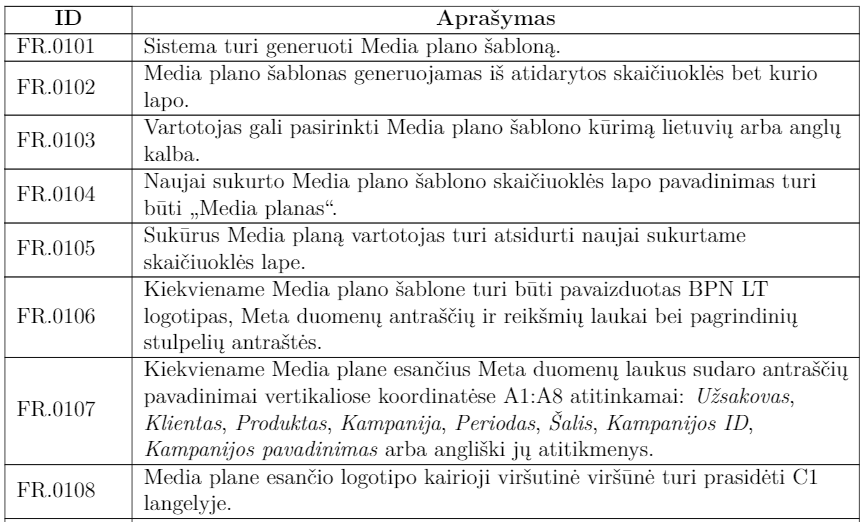
\includegraphics[scale=0.7]{img/reikalavimai}
    \caption{Reikalavimų specifikacijos ištrauka}
    \label{img:model}
\end{figure}

Reikalavimų specifikaciją jau yra tekę pildyti formaliai universitete: Karolio Petrausko kursuose Programų sistemų inžinerija I ir II dalyse bei Sauliaus Ragaišio kurse Programų sistemų kūrimas, todėl ši veikla nesukėlė problemų. Be to, man šis procesas buvo vienas smagiausių praktikos metu ir leido tiksliai aprašyti ko iš sistemos tikisi darbdavys, o ir patys darbuotojai galėjo matyti, koks turėtų būti bendras projekto vaizdas.

Penktoji užduotis buvo prototipo kūrimas. Tai padėjo sužinoti Google Apps Script programavimo kalbos galimybes tam, kad apsibrėžčiau ką įgyvendinti galima, o ką ne, ir jeigu taip, kiek tai turėtų užtrukti laiko. Tačiau Google Apps Script galimybės yra labai plačios ir numačiau, kad  visi apsibrėžti reikalavimai ir norimas pasiekti funkcionalumas yra įgyvendinami apsibrėžtam 5 savaičių laikotarpiui. 

Viena to priežasčių buvo tai, kad Google Apps Script programavimo kalba jautėsi pažįstama, nes ji labai priminė JavaScript programavimo kalbą. Šioje vietoje pravertė universitete įgytos žinios iš Vaido Jusevičiaus kurso Interneto technologijos, į kurį buvo įtraukta šiek tiek JavaScript programavimo kalbos. Perprasti programavimo kalbą nebuvo sunku, todėl rašyti kodą buvo visai paprasta. Be to, dėl panašumų su JavaScript kalba, atsakymų, kurių nepavykdavo rasti Google Apps Script dokumentacijoje ar forumuose, aptikdavau atitinkamose užklausose su JavaScript raktažodžiu.

Sukurtą prototipą parodžiau konsultantams ir šie liko patenkinti, todėl neilgai trukus pradėjau intensyvų sistemos kūrimą.

Kadangi visą projektą teko kurti man vienam ir nuo pradžios, buvo iššūkis suplanuoti efektyvų kodo rašymą perpanaudojant kodą, jį sugrupuojant į modulius ir laikantis to paties kodo standarto. Taip pat siekiau, kad mano programinis kodas būtų lengvai skaitomas kitų žmonių. Toks poreikis kilo, kadangi tikėtina, jog jis bus perduotas BPN LT priežiūrai ir ateityje bus plečiamas kitų praktikantų ar įmonės vidaus specialistų. Galiausiai norėjau laikytis visų gerųjų kodo rašymo praktikų, kad projektas veiktų sparčiai ir efektyviai, o aš įgaučiau kokybiško programavimo patirties.

Projektą pradėjau sukurdamas papildomą pasirinkimą Google Spreadsheets failo meniu juostoje. Paspaudus ant sukurto mygtuko programa sukuria Media plano šablono griaučius. Tai pagrindinių skaičiuoklės laukų reikšmių užpildymas ir stilių nustatymas. Toliau įgyvendinau papildomą funkcionalumą: automatinį įrašų kūrimą, kalendoriaus generavimą ir parašo lauko kūrimą, kurie taip pat buvo pasiekiami per papildomą meniu. 

Automatinis įrašų kūrimas leidžia vartotojui atsidariusiame dialogo lange įvesti norimą kurti įrašų skaičių ir šablone sugeneruojamas atitinkamas kiekis eilučių su nustatytu formatavimu, stiliumi bei formulėmis atitinkamuose laukuose (žr. 3 pav.). Kalendorius generuojamas pagal skaičiuoklėje nurodytą periodo reikšmę, o kalendoriaus laukams pritaikytas sąlyginis formatavimas. Automatiškai sukuriamos mėnesių pavadinimų, savaitės numerių, savaitės dienų pavadinimų ir mėnesio dienų numerių antraštės (žr. 4 pav.). Parašo laukai sukuriami skaičiuoklės apačioje su užpildomais laukais (žr. 5 pav.).

\begin{figure}[H]
    \centering
    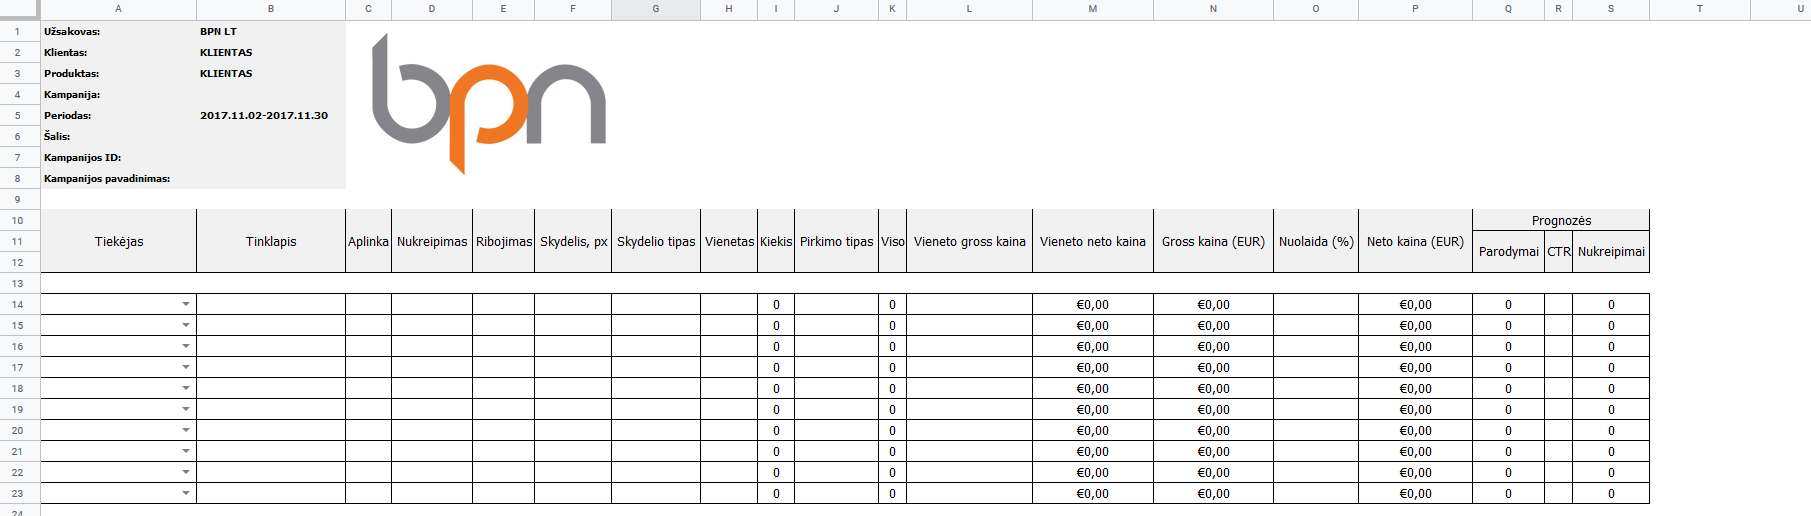
\includegraphics[scale=0.35]{img/generated-records}
    \caption{įvykdytas automatinis įrašų kūrimas}
    \label{img:model}
\end{figure}

\begin{figure}[H]
    \centering
    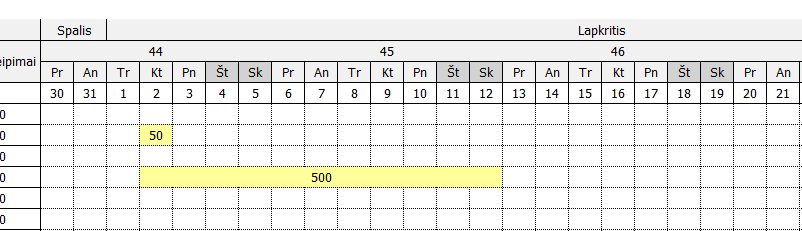
\includegraphics[scale=0.75]{img/records-calendar}
    \caption{Įvykdytas kalendoriaus kūrimas}
    \label{img:model}
\end{figure}

\begin{figure}[H]
    \centering
    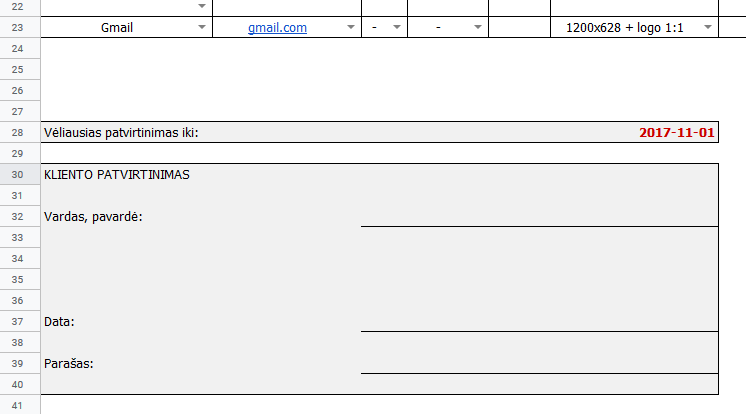
\includegraphics[scale=0.5]{img/signature}
    \caption{Įvykdytas skaičiuoklės parašo kūrimas}
    \label{img:model}
\end{figure}

Šioje vietoje teko susidurti su tam tikrais sunkumais. Generuojant kalendoriaus svaitės dienų antraštes, jos buvo užpildomos lėtai. Tai kėlė neramumų, nes reikalavimų specifikacijoje buvo nefunkcinis reikalavimas, sakantis, kad bet kokia vartotojo pasirenkama atlikti funkcija neturi trukti ilgiau nei 5 sekundes. Kuriant kalendorių su periodu, ilgesniu nei 3 mėnesiai, šis reikalavimas buvo pažeidžiamas. Atlikęs kodo analizę padariau prielaidą, kad to priežastis - cikluose patalpinti Google Apps Script integruoti metodai, skirti darbui su skaičiuoklės langelių reikšmėmis. 

Pasidomėjus internete, mano padaryta prielaida pasirodė esanti teisinga: integruotieji metodai naudoja daug resursų ir paprastai yra taikoma geroji praktika iškelti šiuos metodus iš ciklų arba kaip galima labiau sumažinti jų kiekį cikluose. Mano programinis kodas ir sistemos funkcionalumas nebūtų nukentėjęs, jeigu būčiau iškėlęs dalį šių skaičiavimų iš ciklų, todėl tą ir padariau. Paleidus kodo vykdymą, jautėsi akivaizdus teigiamas programos vykdymo greičio pokytis. Minėtas nefunkcinis reikalavimas buvo patenkinamas nurodžius netgi metų trukmės periodą.

Visas funkcionalumo įgyvendinimas buvo pasiremtas pavyzdiniais vidiniais įmonės šablonais, kuriuos pateikė pati įmonė. Toliau darbai šiek tiek sustojo, nes tolimesnio funkcionalumo įgyvendinimui reikėjo išorinės duomenų bazės. 

Įgyvendinus pradinį funkcionalumą negalėjau pildyti duomenų bazės, nes ją turėjo sudaryti įrašai, kuriuos korektiškai galėjo supildyti tik patyręs BPN LT darbuotojas, dirbęs su dalykine sritimi ilgą laiką. Tam sukūriau atskirą skaičiuoklės failą, kurį pasiekti galėjau aš ir duomenų bazę pildantis asmuo. Sukurtoje duomenų bazėje buvo 70-80 unikalių įrašų su 5 stulpeliais. Šį duomenų bazės failą sinchronizavau su projekto failu, kad pastarasis galėtų pasiekti duomenų bazėje esančius įrašus.

Susiejus projektą su duomenų baze buvo įgyvendintas automatinis įrašų pasirinkimas. Tai yra automatiškai sukurtų įrašų stulpelių užpildymas panaudojant pasirenkamuosius sąrašus su atitinkamų duomenų bazės stulpelių įrašais. Užpildžius pasirenkamojo sąrašo lauką viename stulpelyje, naujas sąrašas atsiranda kitame stulpelyje arba užsipildo automatiškai, jeigu pasirenkamajame sąraše yra tik viena reikšmė. 

Toliau reikėjo įgyvendinti užsakymo šablono kūrimą. Užsakymo šablonas tai pasirinkto kanalo sumažinta Media plano šablono versija, savyje laikanti tik tuos duomenis, kurie yra Media plane. Šis šablonas yra naudingas projektų vadovams norint pamatyti atskirų kanalų užsakymų rodiklius. Užsakymo šablono generavimas paremtas tokiu principu. Kai vartotojas dialogo lange pasirenka norimą kanalą, yra sukuriamas naujas skaičiuoklės lapas, sugeneruojami šablono griaučiai ir nukopijuojamos visos su tuo kanalu susijusio įrašo reikšmės.

Projekto pradžioje buvo sunku numatyti, kaip atrodys galutinis projektas, todėl kodas labai dažnai keitėsi, buvo koreguojama jo struktūra ir grupavimas. Pagrindiniai principai, kuriais rėmiausi atliekant parašyto kodo korekcijas - kuo didesnis patogumas pirmą kartą kodą išvydusiam asmeniui. Pavyzdžiui, programiniame kode ilgą laiką laikiau konkrečias skaitines bei tekstines reikšmes. Asmeniui, analizuojančiam programinį kodą, tos reikšmės nieko nesakytų ir nebūtų galima suprasti, kodėl panaudotos būtent tokios reikšmės ir ką jos reiškia. Taip pat iškiltų problemų norint tuos duomenis pakeisti kitais.

Dėl šios priežasties nusprendžiau sukurti konfigūracinį modulį, kuriame būtų metodai, grąžinantys konstantines reikšmes bei reikšmes, kurios gali keistis priklausomai nuo poreikių. Pavyzdžiui, \textit{Configuration} modulyje buvo metodas \textit{getMediaPlanConstantsEnum}, grąžinantis objektą \textit{mediaPlanConstants}, turintį savyje 14 kintamųjų, kurie, priklausomai nuo projekto ir konteksto, gali būti keičiami. Pavyzdžiui, kintamasis \textit{CALENDAR\_START\_COL\_POSITION} nurodo generuojamo kalendoriaus pradinę stulpelio poziciją, todėl pakeitus metode nurodytą skaitinę reikšmę, pasikeistų kalendoriaus išdėstymo pozicija visame projekte.

Taip pat buvo iššūkis parinkti ribą tarp suprogramuotų ribinių atvejų ir BPN LT darbuotojų sąmoningumo. Parašytas programinis kodas nėra apsaugotas nuo nekorektiško veikimo. Tačiau šis nekorektiškumas atsiranda nuo naudotojo gebėjimo vykdyti instrukcijas. Viena vertus, galėjau suprogramuoti visus įmanomus naudotojo elgsenos atvejus, tačiau tai būtų kainavę per daug mano darbo laiko ir sistemos gebėjimo greitai vykdyti programinį kodą. Kita vertus, to galima išvengti aprašant visus korektiško ir dalį nekorektiško vykdymo scenarijų vartotojo dokumentacijoje ir tikėtis, jog ji bus skaitoma ir vartotojas jos sąžiningai laikysis. Manau didele dalimi pavyko rasti balansą tarp svarbiausių scenarijų suprogramavimo ir dokumentavimo. Prie to prisidėjo mano pasitikėjimas BPN LT darbuotojų gebėjimų lygiu ir sąmoningumu. Galiausiai programinis kodas buvo užbaigtas ir paruoštas testuoti. Iš to sekė šeštoji užduotis.

Šeštoji užduotis buvo programinio kodo perdavimas testuoti. Tam reikėjo tinkamai paruošti projektą. Vienintelis būdas padaryti, kad projektą galėtų testuoti tik BPN LT domene esantys darbuotojai, buvo sukurti Google Spreadsheets plėtinį (angl. \textit{Add-on}). Plėtinio kūrimo procesas buvo labai sudėtingas ir reikalavo daugybės parametrų, tokių kaip prieigos teisių nustatymo, naudojamų išorinių bibliotekų bei daugybės kitų, nurodymo. Čia į pagalbą vėl atėjo dokumentacija, tačiau net ir jos pagalba nepavyko visko tinkamai suderinti, kad plėtinys iš pirmo karto veiktų korektiškai.

Sukūrus veikiantį plėtinį, dalykinės srities konsultantas sukūrė klaidų ir pasiūlymų registrą atskirame skaičiuoklės faile, kurį galėjau pasiekti. Taip pat buvo atrinkti keli BPN LT darbuotojai, kuriems buvo paskirta testuoti mano parengtą projektą. Kol kolegos testavo projektą, pradėjau vykdyti septintą užduotį.

Septintoji užduotis buvo parašyti projekto dokumentaciją. Projekto dokumentaciją taip pat galėjau aprašyti savo nuožiūra, todėl nusprendžiau ją padalinti į 6 dalis: bendra projekto informacija, visos su projektu susijusios šalys, analizės rezultatai, vartotojo dokumentacija, techninė projekto dokumentacija ir autoriaus žodis. Šis dokumentas buvo visa su projektu susijusi medžiaga vienoje vietoje.

Analizės rezultatų skiltyje patalpinau visą reikalavimų specifikaciją su lentelėmis. Vartotojo dokumentacijoje detaliai aprašiau kiekvieną projekte galimą atlikti užduoties scenarijų su nurodymais, rekomendacijomis ir galimomis problemomis. Juos sekė paveikslėliai ir grafinė informacija, turėjusi padėti vykdyti projekte įgyvendintas užduotis. Vartotojo dokumentacija buvo skirta projektų vadovams. 

Techninėje projekto dokumentacijoje patalpinau nubraižytas UML diagramas. Tai užduočių, klasių/modulių bei sekų diagramos. Šioms diagramoms piešti jau turėjau įgytų žinių iš Programų sistemų inžinerijos kurso. Šiame skyriuje taip pat buvo aprašyta detali programinio kodo dokumentacija, aprašanti kiekvienos funkcijos paskirtį, parametrus ir vykdymo seką. Paskutinėje autoriaus žodžio dalyje dokumentavau patarimus ir rekomendacijas įmonei, taip pat dalykus, kurie mano nuomone pravers ateityje projektą pratęsiantiems praktikantams. 

Dokumentacijos rašymas, kaip ir reikalavimų analizė, buvo asmeniškai labai įdomi veikla, išsiskyrusi visame praktikos laikotarpyje. Dokumentaciją rašiau naudodamasis įrankiu \LaTeX, kuriuo išmokau naudotis rašydamas kursinį darbą.

Kol rašiau dokumentaciją, lygiagrečiai stengiausi taisyti kolegų aptiktas klaidas ir įgyvendinti rastus pastebėjimus, aprašytus prieš tai minėtame registro skaičiuoklės dokumente. Dešimtą praktikos savaitę vykdžiau paskutinę užduotį - sistemos diegimą. Diegimui pasirinkau naujausią stabilią programinio kodo versiją. Nors diegimo procesas sutapo su anksčiau minėtu plėtinio sukūrimu, galutinei versijai teko paskirti daugiau laiko ir užduotį atlikti gerokai kruopščiau. Viena to priežasčių - didesnis parametrų kiekis galutinėje plėtinio versijoje. 

Buvo itin svarbu, kad plėtinį pasiektų tik įmonės BPN LT darbuotojai, nes projektas savyje laikė jautrią informaciją. Taip pat reikėjo, kad būtų sutvarkyti įgaliojimai bei prieigos teisės, t.y. kad visi išoriniai failai, kuriuos naudoja projektas, būtų kartu pasiekiami ir visiems BPN LT darbuotojams. 

Galutinis rezultatas buvo toks. BPN LT darbuotojas su BPN LT įmonės paskyra atsidaro naują Google Spreadsheets skaičiuoklės lapą, nueina į Add-ons sekciją ir pasirenka pridėti plėtinį iš oficialios Google plėtinių parduotuvės darbuotojas įsirašo mano sukurtą plėtinį į skaičiuoklę ir po kelių sekundžių pradeda naudotis projektu.

\section{Apibendrinimas}

\subsection{Rezultatai ir išvada}

Galiu išskirti praktikos metu pasiektus rezultatus:
\begin{itemize}
    \item Pasiekti visi praktikos metu išsikelti uždaviniai;
    \item Parašyta apie 1700 Google Apps Script programinio kodo eilučių;
    \item Parengta apie 40 psl. projekto dokumentacijos;
    \item Praktikos metu sukurtas projektas naudojamas įmonės kasdienėje veikloje.
\end{itemize}
\bigskip

Iš rezultatų kylanti išvada - įgyvendinus skaitmeninės reklamos planavimo proceso optimizaciją yra sutaupomas projekto vadovo laikas kuriant skaitmeninės reklamos planą, bei sumažinama klaidų atsiradimo tikimybė skaičiavimuose ar rankinio duomenų įvedimo atveju. Taip yra dėl to, kad tokių duomenų įvedimas sumažintas iki minimalaus, o skaičiavimai atliekami automatiškai, pagal iš anksto aprašytas formules, kurios yra automatiškai įterpiamos generuojant reklamos planavimo šabloną.

\subsection{Praktikos trūkumai ir privalumai}

Nors iš pradžių ir neturėjau didelės motyvacijos atlikti praktikos įmonėje BPN LT, tai buvo įdomi patirtis. Susipažinau su dideliu kiekiu naujų žmonių, išmokau bendrauti darbinėje aplinkoje, jaučiuosi tapęs stipresnis ir atsparesnis ateities darbo paieškose.

Pagrindiniai praktikos trūkumai - neapmokama praktika ir komandinio darbo trūkumas. Taip pat išskirčiau praktikos privalumus. Pavyzdžiui, formalus bendravimas su kolegomis ir darbinės aplinkos pajautimas, kuris manau ateityje pravers dirbant kitose, didesnėse įmonėse. Taip pat labai platus spektras procesų ir užduočių. Praktikos metu turėjau progą išbandyti daugelį projekto gyvavimo ciklo veiklų - nuo planavimo iki diegimo. Dar vienas privalumas - pakankamai modernios technologijos, su kuriomis buvo smagu kurti projektą. Galiausiai lanksčios darbo sąlygos, leidusios į praktiką žvelgti su didesniu entuziazmu.

\subsection{Žinios ir patirtis}

Praktikos metu įgijau programavimo su Google Apps Script, darbo su Google Spreadsheets žinių, praplėčiau planavimo, analizės ir diegimo gebėjimus. Taip pat įtvirtinau turėtą patirtį ir žinias: programavimas HTML, dokumentavimas, komunikavimas, UML diagramų braižymas.

Mano nuomone, universitete įgijau daug naudingų žinių ir tam tikrą filosofiją, požiūrį į atliekamą veiklą bei savarankišką mokymasį. Dėl šių priežasčių nesusidūriau su neįveikiamais sunkumais atliekant praktikos metu paskirtas užduotis ir darbus. Taigi, universitete įgytų žinių atitikimą praktikos užduočiai atlikti vertinčiau labai gerai.

\subsection{Pasiūlymai}
Turiu kelis pasiūlymus mane į praktiką priėmusiai įmonei. Visų pirma, manau, kad mokamas atlyginimas praktikos metu, net ir minimalus, žymiai labiau paskatintų stengtis siekti rezultatų. Vis dėlto įmonės priima IT srities studentus, todėl tikėtina, kad jis sukuria nemažą pridėtinę vertę savo praktikos rezultatais, kuria įmonė neatlygintinai naudojasi savo ateities veiklose. Pavyzdžiui, aš automatizavau ir optimizavau projekto vadovo veiklą, kuri paprastai užima didelę dalį projekto vadovo darbo laiko. O tai reiškia sutaupytus pinigus, kuriuos pasiima įmonė ir prarastus pinigus studentui, kuris tokį patį dalyką galėjo sukurti kitoje įmonėje ir už tai gauti atlygį. Taigi, mano siūlymas būtų skirti bent minimalų atlyginimą arba premiją už pasiektus ir įmonei naudingus rezultatus.

Kitas pasiūlymas būtų labiau pasiruošti priimti praktikantus. Mano atvykimo metu jautėsi šiokia tokia sumaištis dėl to, ką turėsiu daryti praktikos metu. Jautėsi nesusitarimas tarp vadovų, o užduotys buvo paskirtos nepaaiškinant nei ką konkrečiai sukurti, nei koks detalus jų atlikimo planas. Tiek planavimo, tiek analizės procesus turėjau pasiūlyti pats, kas manau išgelbėjo praktiką nuo katastrofos. Visa ši sumaištis taip pat buvo priežastis to, kad viduryje praktikos, kovo mėnesį, teko keisti praktikos temą bei uždavinius. O tai sukėlė papildomų rūpesčių, laiko ir nervų sąnaudų. Buvo dar apmaudžiau ir dėl to, kad darbo pokalbyje sutarta ir pažadėta veikla nesutapo su mano praktikos laikotarpiu konkrečiai vykdoma veikla, todėl jaučiausi šiek tiek apgautas įmonės. Mano siūlymas būtų prieš paskelbiant apie praktikos poziciją, įmonė turėtų aiškiai ir konkrečiai apsibrėžti lūkesčius, ką praktikantas turės atlikti, kas jį prižiūrės, bus atsakingas už rezultatus ir nuosekliai laikytis pažadų.

Dar vienas siūlymas būtų susijęs su praktikos vykdymu. Aš visą laiką dirbau individualiai. To nelaikau didžiuliu trūkumu, nes galėjau įrodyti ir parodyti savo kompetencijas bei prisiimti visišką atsakomybę už atliekamus darbus. Tačiau jaučiu, kad neįgavau darbo komandoje patirties, kurios norėjau. Taip pat susidarė įspūdis, kad niekam be manęs praktika ir mano rezultatai nebuvo įdomūs. Didžiąją dalį pokalbių, susijusius su praktika, turėjau inicijuoti aš, klausimai taip pat kildavo iš mano pusės. Mano siūlymas būtų praktikos vadovais skirti motyvuotus, atsakingus ir iniciatyvius darbuotojus.

Taip pat turiu kelis pasiūlymus universitetui. Viena iš problemų - nelygybė atsiskaitymų metu. Pastebėjau, kad praktinių užsiėmimų dėstytojai labai skiriasi ir jų vertinimai iškraipo bei destabilizuoja realią situaciją. Dažnai pasitaikydavo modulių, kai vienas pogrupis gaudavo griežtą dėstytoją ir jis ženkliai numušdavo visų balus, programų atsiskaitymai labai vargindavo ir trukdavo kelias savaites, o kitas pogrupis gaudavo dėstytoją, kuris už bet kokį darbą rašydavo maksimalų įvertinimą tą pačią paskaitą. Panaši situacija ir su egzaminais arba gynimais - nelygaus kalibro variantų užduotys ir komisijų nariai. Egzaminų klausimu būtų galima organizuoti suvienodintus egzaminus kompiuterių auditorijose Saulėtekyje.

Manau, kad į studijų programą reikia įtraukti žymiai daugiau su Programų sistemomis susijusių modulių. Nors ir manau, kad studijų programos planas yra subalansuotas tikrai gerai, tačiau pasigedau daugiau modulių apie projektų valdymą, programinės įrangos inžineriją, architektūrą, kurie man asmeniškai pasirodė vieni įdomiausių. Manau šių modulių sąskaita būtų galima paaukoti dalį C grupės pasirenkamųjų dalykų.

Taip pat į studijų planą būtų galima įtraukti stipresnį mokslinių darbų rašymo modulį, nei Profesionalumas ir etika. Akivaizdu, kad kursinių ar baigiamųjų darbų rašymas yra vienas labiausiai pastangų pareikalaujantis darbas, kurio rašymui studentai nebūna labai gerai paruošti. Vargsta net ir gabiausi studentai. Mano siūlymas būtų išskirti tam daugiau kreditų arba sustiprinti esamą Profesionalumo ir etikos modulį.

Dar vienas siūlymas - perteikti arba parodyti darbdaviams studijų naudą. Šiuo metu beveik niekas neturi motyvacijos skirti savo laiko rimtai akademinei veiklai arba siekti aukštų akademinių rezultatų. Viena to priežasčių - dalis pradeda dirbti pirmame kurse gerai apmokamose vietose, augina savo patirtį ir kompetencijas šitaip dar labiau pasididindami savo atlyginimą. Tuo tarpu gerai besimokantys studentai gauna 57 arba 95 eurus stipendijos per mėnesį, neaugina praktinių gebėjimų ir po studijų uždirba gerokai mažiau, nei tie, kurie studijų pastangas paaukojo darbui. O tai mano nuomone yra tam tikras pasityčiojimas. Darbdaviai, suprasdami studijų svarbą ilgojoje perspektyvoje, vengtų darbinti ankstyvųjų kursų studentus ir labiau vertintų studijas pabaigusius studentus.

Privalomos praktikos modulyje iš anksto paskirti praktikos vietą studentui. Praktikos paieškos metu žiemą ieškojimo procesas suvalgė daug laiko, nervų ir pastangų, nes rasti praktikos vietą buvo be galo sunku, o kartais apimdavo neviltis ir atrodė, jog teks gauti skolą už profesinę praktiką. Būtų žymiai paprasčiau, jei būtų galima pasirinkti, kad universitetas paskirtų praktikos vietą savo nuožiūra.

Dar vienas siūlymas - privalomai apmokama praktika. Studentai, neieškoję darbo ir baigę studijas, yra išleidžiami į gatvę. Baigus studijas jie neturi nei gyvenamosios vietos, nei darbo. Vilniuje pragyvenimas nėra labai pigus, todėl būtų logiška, jei tie 2-3 mėnesiai, kuriuos studentas praleido praktikuodamasis, konvertuotųsi į piniginį formatą bent minimalios algos forma ir būtų išmokami sėkmingai apsigynus baigiamąjį darbą, tarsi socialinė išmoka gyvenimo pradžiai: butui išsinuomoti ir išgyvenimui pirmiesiems mėnesiams darbo rinkoje.

Kitas siūlymas būtų priimti mažiau studentų į Programų sistemų studijų programą bei kitas, tokias kaip informatika. Tai gali pasirodyti kaip labai keistas siūlymas, tačiau bendraudamas su kursiokais ar IT srities žmonėmis pastebiu, kad nors šiuo metu darbo rinkoje ir yra patyrusių specialistų trūkumas, tačiau yra pradinio lygio IT specialistų perteklius (baigę studijas, akademijas ir beveik neturintys darbo patirties). Tai labai apsunkina darbo paieškas ir numuša atlyginimus. To privalumas būtų tai, kad studijuoti būtų priimti tik patys gabiausi studentai ir sumažėtų studijas nebaigiančių ar net metančių žmonių.


%--------------------------------------------------------
%----------------------- PRIEDAI ------------------------ 
%--------------------------------------------------------

\end{document}